\documentclass[12pt]{paper}



\usepackage[margin=1in]{geometry}
\usepackage{tikz}
\usepackage{natbib}
\usepackage{amsmath}
\usepackage{bm}
\usepackage{amsthm}
\usepackage{mathtools}
\usepackage{amsfonts}
\usepackage{bbm}
\usepackage{graphicx}
\usepackage{tabularx,ragged2e,booktabs,caption}

\renewcommand{\arraystretch}{1.2}

\DeclareMathOperator{\diam}{diam}
\DeclareMathOperator{\interior}{int}
\DeclareMathOperator{\close}{cl}

\newcommand{\met}[1]{d \left ( #1 \right )}
\newcommand{\brak}[1]{ \left [ #1 \right ] }
\newcommand{\cbrak}[1]{ \left \{ #1 \right \}}
\renewcommand{\vec}[1]{ \bm{ #1 }}
\newcommand{\abs}[1]{\left \lvert #1 \right \rvert}
\newcommand{\seq}[1]{{\left \{ #1 \right \}}}
\newcommand{\conj}[1]{ \overline{ #1 } }
%\newcommand{\close}[1]{ \bar{ #1 } }
\newcommand{\set}[1]{\left \{ #1 \right \}}
\newcommand{\Lim}{\lim\limits}
\newcommand{\compose}{\circ}
\newcommand{\inv}[1]{{#1}^{-1}}
\newcommand{\compl}[1]{{#1}^{c}}



\newcommand{\setR}{ \mathbb{R} }
\newcommand{\setQ}{ \mathbb{Q} }
\newcommand{\setZ}{ \mathbb{Z} }
\newcommand{\setN}{ \mathbb{N} }

\newcommand{\plim}{ \overset{p}{\to} }
\newcommand{\mean}[2][N]{ \overline{ #2 }_{#1}}
\newcommand{\exV}[1]{\mathbb{E} \left [ #1 \right ]}
\newcommand{\Vari}[1]{\mathbb{V} \left ( #1 \right )}

\newcommand{\est}[2][n]{ \widehat{ #2 }_{#1}}
\newcommand{\altest}[2][n]{ \tilde{ #2 }_{#1}}

\newcommand{\indicate}[1]{ \mathbbm{1}_{\{#1\}}}
\newcommand{\convDist}{ \overset{d}{\to}}
\newcommand{\unif}{\emph{U}}
\newcommand{\normal}{\mathcal{N}}
\newcommand{\eye}{\mathbbm{I}}

\newcommand{\bigO}{\mathcal{O}}
\newcommand{\Lagrange}{\mathcal{L}}

\newcommand{\deriv}[2]{\frac{ \partial #1}{ \partial #2}}

\DeclarePairedDelimiter{\ceil}{\lceil}{\rceil}
\DeclarePairedDelimiter{\floor}{\lfloor}{\rfloor}
\DeclarePairedDelimiter{\norm}{\lVert}{\rVert}

\newtheorem{assume}{Assumption}

\bibliographystyle{chicago}

\title{The Longshot bias in market data: Evidence from Counter-Strike:
  Global Offensive}
\author{Timothy Schwieg}

\renewcommand\maketitle{}
\begin{document}

\maketitle
\bibliographystyle{chicago}

\begin{titlepage}
\centering
{\scshape\LARGE University of Chicago\par}
\vspace{1cm}
{\scshape\Large MACS 40200\par}
\vspace{1.5cm}
{\huge\bfseries The Longshot bias in market data: Evidence from Counter-Strike:
  Global Offensive\par}
\vspace{2cm}
{\Large\itshape Timothy Schwieg\par}
\vfill
\justify
In this paper I investigate whether or not behavioral models of
behavior under uncertainty explain market level sales of
lotteries. I extend a homogeneous model of logit demand in the a
characteristic space to several functional forms of the valuation
function for a lottery. The data come from online sales of lotteries
in a complete market for video game cosmetics. These lotteries contain
many low probability and high value contents. I find that the
behavioral model of cumulative prospect theory does no better at
explaining variation in the market shares than a rational model. I
find that the rational model does do better at describing equilibrium
between the prices of the contents and the prices of the lotteries
that contain these contents. 
\vfill
\centering
{\large \today\par}
\end{titlepage}


\section{Introduction}

Many structural models for individuals behavior have lost popularity
among applied economists because of strict assumptions of rationality
on behavior. In this paper I examine a relaxation of this behavior and
investigate whether or not it can be used to explain behavior better
than other rational models.  I hope to shed light on a question of
whether a class of behavioral models, cumulative prospect theory, is
helpful in considering selling mechanisms that utilize randomness. I
use field data from a collection of markets for lotteries as well as
secondary markets for each of their contents to determine valuations,
and build a model of risk preferences from this. I seek to answer the
question of whether or not this model provides additional predictive
and explanatory power in examining behavior of individuals buying
lotteries. I aim to analyze which components of this model of behavior
are most important in these lotteries being valued so much above their
expected value.

The question of interest is whether or not Cumulative Prospect theory
is able to better explain decision making in low-risk lotteries than
Expected Utility theory, and if so, what mechanism allows for this
better explanation. In particular, the robustness of the parameters in
terms of their out-of-sample fit is also of interest, as different
researcher's calibrations of the model have found quite different
results. 

In essence, I have a field experiment and wish to determine from this
data whether or not cumulative prospect theory can explain
individual's behavior better than traditional ``rational'' models of
consumer behavior. This is an ideal setting for such a project as
these lotteries combine many elements that behavioral economists would
term "irrational". These lotteries feature many high value but
extremely low (order of $10^{-5}$) probability outcomes, the potential
market is mainly teenagers, and the cost of participation is low
(\$2.50-4.00). In such a setting, one would expect a large gain from
predictive power employing a behavioral model of risk.

If there are indeed large gains to be had from considering this
behavioral model over the expected utility framework, it may be that
many behavioral notions of irrationality, such as bidding behavior in
auctions can be explained. To generalize these results from
small-scale lotteries to distinct fields such as auctions, there must
be some notion of robustness of the parameter estimates, and I intend
to investigate whether or not these parameters are dependent on the
structure of the lottery, or are primitives in the purest sense. 

This question is relevant to the larger field of Industrial
Organization because it is able to bring the question of preference
heterogeneity previously studied by \cite{Snowberg2010} among others
in horse betting. We are able to abstract ourselves from the concerns
of belief heterogeneity suggested by \cite{Gandhi2014} due to the
specific structure of the market, and thus are able to isolate the
effects of only preferences. I extend this notion to market
data. Previously the literature had been focuses on contracts, whether
in betting markets or in financial markets.

While the data is focused on sales in online markets for video game
items. This type of mechanism is not limited to this market
only. Randomization mechanisms are popular ways of selling collectible
items and trading cards in both virtual and actual markets. This same
type of mechanism is also present in less-fringe markets such as
children cereal collectibles and toys in fast-food kids meals. Each of
these markets attempts to exploit the ``irrationality'' of children's
behavior under uncertainty. We attempt to study this focusing on
market data where valuations for each of the contents as well as the
lottery are represented from a market. However these results can be
extended to any type of market where randomization is the primary
selling mechanism. 


\section{Literature Review}

\cite*{LitReview} presents a broad review of where Prospect theory has
been applied, as well as its problems with its application,
particularly in the choice of a reference point, which appears to be
very significant, but there is little guidance on what to choose
beyond possibly the expected value of the lottery. Applications of the
model, originally proposed by \cite*{Kahn} exist mostly in finance and
insurance. I intend to extend this body to look at the behavior of
non-expert individuals in a market scenario. I believe that this area
has not had many applications, likely because of the rarity of quality
data outside of these fields.

The literature on Cumulative Prospect theory, the main structure of
this model is primarily focused on experimental data. The literature
began with the paper by \cite*{ProspectTheory} that suffered from
problems relating to stochastic dominance, and was updated in 1992
with their paper on cumulative prospect theory. 

\cite*{GONZALEZ1999129} give a discussion on the interpretation and
development of the probability weighting function used in cumulative
prospect theory as well as several forms and their ensuing
interpretations. The different parameters are identified with respect
to psychological phenomena found relevant to the decision making
process. Thus ``identification'' in the reduced-form sense of
interpretation of the parameters become much more possible, as there
are many dimensions of the model.

The work on the application of Cumulative Prospect Theory within
industrial organization has been limited, likely due to poor data. One
area where the data has been rich has been horse betting, and
\cite{Snowberg2010} applies cumulative prospect theory in a
non-parametric setting to this data to explain the long-shot bias
present there. There are also lots of applications in financial
markets where there is better data, one such example is \cite*{Thaler1995}.
\cite*{Sydnor2010} presents an application of prospect theory to real-world
data. He uses data on homeowner's choices on deductibles for
home-insurance policies as a measure of moderate financial risks. The
main body of the paper focuses on the standard expected utility
framework, but it is extended to cumulative prospect theory in a
discussion. There is however no empirical work with prospect theory on
the data, as there is substantial heterogeneity within the data.

\cite*{Barseghyan2012} form a structural model based on a discrete
choice model, and non-parmetrically estimate the utility function as
evidence for the existence of probability weights in insurance
choices. This can be explained by cumulative prospect theory's
decision weighting scheme. Much of the literature on experiments in
this field also shows that the results are sensitive to the
experimental conditions, \cite*{PlottZeiler}

\cite{LitReview} discuss the use of preference for lottery-payoffs for
encouraging behaviors, which is relevant to my market. However the
literature is underdeveloped, likely due to its legal nature in the
United States.

This paper builds on some literature in the Industrial Organization
Field that is based around applying behavioral models to structural
estimation. \cite*{BajariHortacsu2003} examine whether or not traditional
models of auction behavior can explain auction bidding behavior
compared to adaptive models of learning and quantal response
equilibrium. However, rather than examining experimental data to draw
conclusions, I intend to use field data. \cite{Gandhi2014} examines
the long shot bias in financial data again, but uses belief
heterogeneity rather than preference heterogeneity. 

The demand estimation framework that I intend to employ is the
discrete-choice demand framework introduced by McFadden (1971). This
paper was extended to demand estimation with a shock in \cite{Berry1994}
that is the model I intend to emulate for my discrete choice
estimation. Heterogeneity was introduced into this framework in the
seminal paper by \cite*{BLP} that develops the multinomial logit
demand system that is common in demand estimation today. This
alleviates some of the theoretical problems that are created by the
structure of the discrete choice estimation, namely independence of
irrelevant alternatives. 

There is a focus on using Discrete choice models with prospect theory
that has appeared in the Travel Behavior Literature. Such as
\cite{LiHensher2011} and \cite*{dePalma2007}. This literature,
inspired by \cite*{dePalmaEtAl}, uses different behavioral models of
individual behavior under lotteries directly in the utility
specification of discrete choice. The paper discusses the different
function forms and choices made by the researched in choosing the
behavioral model to estimate choices.  The emphasis on the behavioral
models, is on improving prediction rather than better explanatory
power for the model. In particular, all of these exercises use
simulated data or laboratory experiments to evaluate consumer's
decision making, rather than estimating parameters from market choices
that are observed. These problems manifest themselves in a lack of a
measure of willingness to pay as well and reference point, making
estimation of the parameters difficult when it is even attempted. This
existing literature on transport fails to address individual specific
heterogeneity as well.


\section{Data}

The Data come from the \emph{Steam Community Market}, a system of
continuous double auctions that operates as a competitive
market. Individuals place buy and sell orders which are then matched
according to the seller's price. The lotteries of interest are sold on
the market, and each of their contents are sold individually as
well. Since this structure of a market converges quickly to a
competitive equilibrium, we have high quality data on the equilibrium
price and quantity of not only the lottery, but for each of its
contents. The specific data examined are market transaction history
for all items sold on the \emph{Steam Community Market} for
Counter-Strike: Global Offensive.

Counter-Strike Global Offensive is a first-person shooter game where
one team (terrorists) attempt to plant a bomb and defend it while the
counter-terrorists attempt to defuse the bomb. Each team has specific
guns that they are able to purchase at the start of every round. The
in-game cost, game balance, and meta-game all contribute to the
popularity of each weapon. Players may choose to purchase purely
cosmetic ``skins'' for their weapons which change the appearance of
their weapon when they buy it. These skins are sold in lotteries
called weapon crates which are dropped randomly to players
in-game. The drop rates are unknown, and believed to change
often. Upon receiving a weapon crate, a player may elect to spend
\$2.50 to open it, or sell it on the community market.

These crates display which weapon skins they may contain, and the
probability of obtaining each item within the crate is public
knowledge, as required by Chinese Law. That is, the contents of the
crate follow a known distribution, and can therefore be estimated
under theories of risk. The contents of the crate can then be held
onto, or sold at market.
 

\subsection{Market}


The market that these weapons can be sold at is the \emph{Steam
  Community Market} which is run by Valve, the same company that makes
Counter-Strike: Global Offensive. The market is a continuous time
double-auction. Sellers may place sell orders, and buyers buy orders,
and the market functions by matching the buyers and sellers, always
selling at the seller's price. This is known to converge quickly to a
competitive market, and will be treated as such for this
project. \cite{Efficiency} There are two complications however, there is a 15\% tax
placed on the market by Valve, which is taken from the seller's
earnings. This is complicated by the discrete nature of the selling,
and the tax always rounds up in favor of Valve. That is, an item
selling for \$0.03 would return \$.02 to Valve rather than 15\%. This
will not be a large factor in my model as I am primarily interested in
calculating demand.

For the past 30 days, there is data on hourly median market price as
well as quantity sold. For the remaining time that an item has been at
market, there is data for daily median price and quantity sold. The
data also contain active buy and sell orders at the time of its
mining: (June $7^{th}$ 2018). No history for these buy and sell orders
is available.

From this data, the expected value of the lottery under various forms
of utility functions can be calculated, as the prices of all of the
contents are given in equilibrium with the prices of the lotteries
themselves. A graph of the expected values against the prices of
opening the lotteries is given below, using the number of contents of
each of the lotteries as the temperature.

\begin{center}
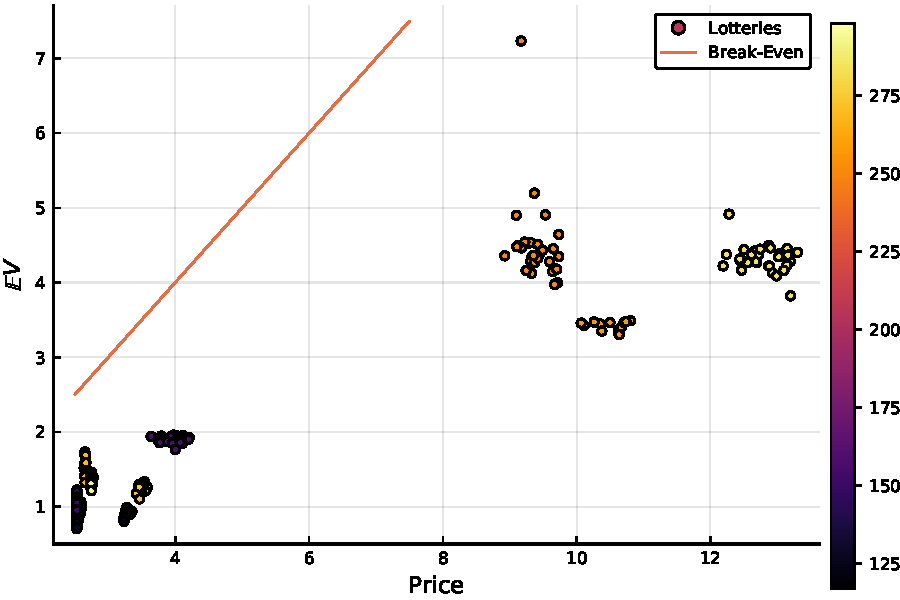
\includegraphics[width=.9\linewidth]{../Plots/BreakEvenScatter.pdf}
\end{center}

Thisgraph demonstrates the clustered nature of these boxes, indicating
that there is not a large amount of price variation overall. It also
motivates the use of characteristic space models as the different
lotteries appear to be quite clustered together with their own data
points.


This graph suggests that there may be a link between the size of the
lottery and the number of losses, and this is investigated in the next
graph.

\begin{center}
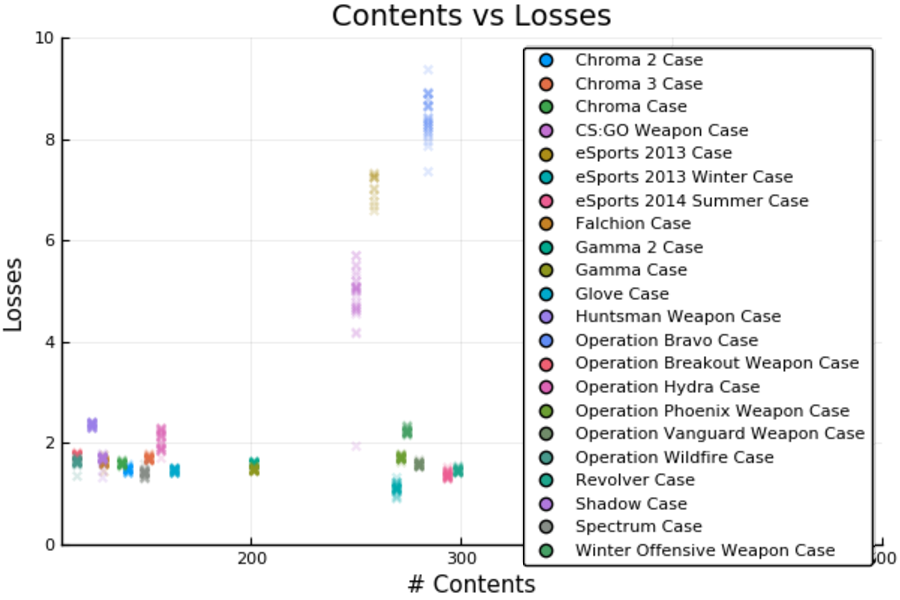
\includegraphics[width=.9\linewidth]{../Plots/LossesVSize.pdf}
\end{center}

Here we can see that although a large expected loss means that there
are many contents of the lottery, the converse is not shown in the
data. 

\subsection{Characteristics}

Since the model used will be in the characteristic space rather than
the product space, I am especially interested in characteristics of
the different weapons in the game. I shall ignore the characteristics
that will be used to determine the market for the weapon, detailed in
Assumption 1 in the model section. Unique to each weapon is a float
value, between $0$ and $1$, which indicates the wear on the
weapon. Wear does not change with use, and is determined when a weapon
is un-boxed. This float is distributed uniformly, but based on its
value, places the weapon into different brackets for sale. We will
consider all weapons in a particular bracket as homogeneous. The
contents of the crate are divided into several tiers based on their
rarity from being obtained in a box. All of the statistics of a
particular item that can be unboxed are summarized in the tables
below.


\begin{table*}[!htb]
    \begin{minipage}{.5\linewidth}
      \caption{Condition Probabilities}
      \centering
        \begin{tabular}{|l|l|}\hline
          Float & Condition\\\hline
          0.00 - 0.07 & Factory New\\
          0.07 - 0.15 & Minimal Wear\\
          0.15 - 0.38 & Field-Tested\\
          0.38 - 0.45 & Well-Worn\\
          0.45 - 1.00 & Battle-Scarred\\\hline
\end{tabular}
    \end{minipage}%
    \begin{minipage}{.5\linewidth}
      \centering
        \caption{Rarity Probabilities}
        \begin{tabular}{|c|l|}\hline
          Probability & Rarity\\\hline
          .0026 & Special (Gold)\\
          .0064 & Covert (Red)\\
          .032 & Classified (Pink)\\
          .1598 & Restricted (Purple)\\
          .7992 & Mil-spec (Blue)\\\hline
\end{tabular}
    \end{minipage} 
\end{table*}

Independent of wear, each item
also has a $10\%$ chance of being StatTrak\texttrademark, where the
gun includes a tracker that counts the number of kills a player has
with this weapon. This number is reset on sale, so it can be treated
simply as a binary indicator.

Conditioned on the rarity, there are still many variants of the
contents available, and there is substantial heterogeneity in the
amount of contents in each of these brackets. The largest amount of
heterogeneity is in the Gold tier.  Several of these lotteries have in
excess of a hundred possible contents, reaching a maximum of 228 items
in the gold tier. This leads to an extremely large amount of items
with extremely low probabilities of being unboxed. This provides a
distinction between two groups of lotteries, ones with many rare
items, and the others where they are distributed evenly among the
brackets.

\begin{minipage}{\linewidth}
  \centering
  \captionof{table}{Lottery Details}
  \begin{tabular}{@{}lcccccccc@{}}\toprule
    & \multicolumn{2}{c}{Values} & &\multicolumn{5}{c}{Number of Contents}\\
    \cmidrule{2-3} \cmidrule{5-9}
  Case & $\mathbb{E}[V]$ & Price &\quad& \#Blue & \#Purple & \#Pink & \#Red & \#Gold\\\midrule
Operation Wildfire  & 0.89891 & 2.5307 &\quad& 26 & 18 & 14 & 9 & 50\\
Operation Breakout  & 0.77011 & 2.5305 &\quad& 24 & 15 & 12 & 10 & 56\\
Falchion Case  & 0.95072 & 2.5323 &\quad& 27 & 24 & 11 & 9 & 59\\
Shadow Case  & 0.85299 & 2.5349 &\quad& 29 & 17 & 14 & 10 & 59\\
Huntsman Weapon Case  & 0.95531 & 3.3181 &\quad& 25 & 17 & 12 & 8 & 62\\
Spectrum Case  & 0.98146 & 2.53 &\quad& 34 & 23 & 15 & 9 & 68\\
Chroma 2 Case  & 1.0058 & 2.53 &\quad& 25 & 13 & 13 & 9 & 81\\
Chroma 3 Case  & 0.66099 & 2.53 &\quad& 30 & 19 & 11 & 10 & 81\\
Chroma Case  & 0.83215 & 2.55 &\quad& 23 & 20 & 10 & 4 & 81\\
Glove Case  & 0.84301 & 2.53 &\quad& 27 & 26 & 9 & 12 & 89\\
Operation Hydra  & 1.5465 & 4.0827 &\quad& 25 & 20 & 14 & 9 & 89\\
Gamma 2 Case  & 0.68335 & 2.53 &\quad& 31 & 22 & 13 & 7 & 128\\
Gamma Case & 0.80717 & 2.53 &\quad& 31 & 21 & 11 & 10 & 128\\\hline
CS:GO Weapon  & 4.4611 & 9.3248 &\quad& 7 & 6 & 7 & 2 & 228\\
eSports 2013 Case  & 3.2708 & 10.354 &\quad& 8 & 13 & 7 & 2 & 228\\
eSports 2013 Winter  & 1.5687 & 2.6441 &\quad& 18 & 9 & 11 & 3 & 228\\
eSports 2014 Summer  & 1.4136 & 2.7414 &\quad& 21 & 19 & 16 & 9 & 228\\
Operation Bravo  & 4.3567 & 12.628 &\quad& 26 & 15 & 9 & 6 & 228\\
Operation Phoenix  & 0.85507 & 2.5416 &\quad& 15 & 12 & 9 & 7 & 228\\
Operation Vanguard  & 1.038 & 2.5928 &\quad& 17 & 13 & 12 & 10 & 228\\
Revolver Case  & 1.1045 & 2.53 &\quad& 24 & 25 & 12 & 9 & 228\\
Winter Offensive  & 1.299 & 3.5079 &\quad& 14 & 14 & 12 & 6 & 228\\\bottomrule
  \end{tabular}
  
\end{minipage}

\section{Model}



\subsection{Discrete Choice Demand}

Let us believe that individuals have a valuation for loot boxes
characterized by some function $V(.)$. Following a discrete choice
framework for demand estimation, I assume that the utility of a
consumer $i$ for loot box $j$ in time $t$ is given by:
\begin{equation*}
  u_{ijt} = V( x_{jt}, p_{jt}; \theta ) + \xi_{jt} + \epsilon_{ij} \quad \epsilon_{ij} \sim Gumbel
\end{equation*}

Where $p_{jt}$ is the price, $x_{jt}$ are the covariates, $\xi_{jt}$ is
some demand shock common to all consumers (this can be rationalized as
unobserved benefits), $\epsilon_{ij}$ is a type-1 extreme value shock unique
to the consumer and good, and $\theta$ is the vector of parameters for the
valuation function

The demand for this good then is given by the probability that it has
the maximum utility. This can be computed using the properties of the
Type-1 extreme value distribution. The maximum follows a logistic
distribution, and the probability is given by:

\begin{equation*}
  \Pr( i \rightarrow j ) = \frac{\exp( V(x_{jt},p_{jt} ; \theta) + \xi_{jt})}{ \sum_{k \in \mathcal{F}}
    \exp(V(x_{jt},p_{jt}; \theta) + \xi_{kt})}
\end{equation*}

In this sense, demand is non-random, and the Econometrician observes
the price of the box, the covariates of the box, as well as the
equilibrium quantity $q_{jt}$. All facets here observed, save the fact
that the price and quantity are equilibrium prices and quantity rather
than various points along the same demand curve.

Following the structure of \cite{Berry1994} we consider an outside option
that has some market share. The outside option is simply not partaking
in any of the lotteries, and thus the valuation of this is $0$.
However there is still some unobserved demand $\xi_{0t}$. Inversion to
solve for this parameter is simple, as
$\Pr( i \rightarrow 0) = \frac{1}{ \sum_{k \in \mathcal{F}} \exp(V(x_{jt},p_{jt}; \theta) +
  \xi_k)}$.  Dividing each demand equation by the outside option and
taking logs yields us:

\begin{equation*}
  \log s_{jt} - \log s_{0t} = V(x_{jt}, p_{jt}; \theta) + \xi_{jt}
\end{equation*}

Since $\xi_{jt}$ is unobserved by the econometrician, it takes the form
of the unobserved error in the demand estimation procedure. However,
it is sometimes endogenous to price as price is formed by the
intersection of both supply and demand shocks. We need valid
instruments for the estimation of this demand.

\subsection{Instruments}

Endogeneity occurs in this model via the simultaneity of supply and
demand. Valid instruments for the price therefore must be supply
shifters that do not affect the demand. Supply can be thought of as
the players who have received a loot box randomly and wish to sell
it. To simplify the dynamics of the problem, upon receiving the item
individuals plan to sell it or not, so the supply of these loot boxes
is heavily dependent on active players in that day and the previous
day. 

It is assumed that demand is a function of the long-run average number
of players, or the amount of ``active players'' over the period of the
month. This number is different from the daily players that play each
day, as relatively few people are able to play each day for many
reasons. However, loot boxes are given randomly to each player who
plays in a day. We wish to use this fact to construct instruments for
the demand. Suppose the true number of active players is $N$. Then daily
players is $N + \epsilon_t$, i.e. some shock that determines daily
player-base. We wish to use this shock $\epsilon_t$ as a cost-shifter that
does not affect demand. If we estimate N by the average of all players
over a significant time period, we can instrument demand using the
daily deviations from this average. We instrument for price with the
deviations of the current day of sale as well as the previous days.


Supply can be thought of as upward sloping with an active price floor
at a price of $.03$ which is often binding. In the set of transactions
where the price floor is binding, there is no concern of simultaneity,
and therefore price is exogenously determined by the existence of the
price floor. Since we use multiple instruments for price in the
endogenous case, the remaining instruments will be made zero for the
exogenous price case. 

Demand can then be estimated off of the condition that:
\begin{equation*}
  \exV{Z_t (\xi_{tj})} = 0 \quad \quad \quad \exV{ p_{jt} \xi_{jt} } = 0 \quad \text{When } p = \$.03
\end{equation*}

Also present in the data is active buy orders, these are orders
that there is not yet supply to fulfill. However it is a dominant
strategy for place your valuation as the bid. Therefore there is no
concerns about shading, and we may treat these orders as true
valuations. In the case of these estimates, we should find that demand
shock is equal to zero, and uncorrelated with the valuation, or that
$\exV{p_{jt}\xi_{jt}} = 0$. I note that the same choice and discrete
choice framework holds for those that post unfulfilled buy orders, so
there is no different model for valuations under the unfulfilled order
framework. 

This gives us instruments to identify price effects for each of the
possible cases of the data. The other exogenous covariates present in
the model 


The rest of the covariates are the
probabilities of obtaining each of the items, which are obviously
exogenous and the last known prices of the contents of the loot
boxes. We shall takes these prices as exogenous as they were
determined by the supply and demand of the item in previous time
periods. In this sense we are completely abstracting the problems from
dynamic choices regarding optimal opening of boxes or strategies in
continuous time double auctions. 

We may combine all of these into a vector $x_{jt}$ along with a
constant term and our condition becomes one of
$\exV{x_{jt}\xi_{jt}} = 0$. This provides us with $k + 3$ moments per
data point, when there are $k$ contents, and there are $3$
parameters of interest to estimate. We are extremely over-identified,
allowing for the possibility of more complicated functional forms such
as splines as extensions. 




\subsection{Cumulative Prospect Theory}


We now examine the structure of the Valuation function $V( x_j,
p_j; \theta)$. Denote the probabilities of each of the contents of the
lotteries by $\pi_i$ and their values as $x_i$. We now re-index these by
a permutation $s_i$ such that $x_{s_1} < x_{s_2} < ...$ and so on. The
cumulative probability $\Pi_i$ can be written as $\sum_{i=1}^K
\pi_{s_i}$. From these objects we can construct the value function for
the lottery.

Cumulative Prospect Theory includes several important concepts not
observe in classical decision making under risk. It incorporates
reference dependence, which implies that people view things in the
context of losses and gains rather than changes to their overall
wealth. This is attractive for computational reasons. It also utilizes
loss aversion, the notion that losses are relatively more costly than
gains. The model also incorporates diminishing sensitivity, the notion
that valuations are concave in losses and convex in gains. The final
concept is probability weighting, the notion that consumers act as if
they were facing different probabilities than what they encounter.

We note that the price of opening a case is two-fold, first the case
must be bought at the market for its price, and then the price of the
key, denoted $p_{key}$ must also be paid to open the case. The time
required to open the case is trivial, and will not be
considered. Since gains are treated differently than losses, let the
parameterization of these gains and losses be defined as:

\begin{equation*}
  v(x) =
  \begin{cases}
    x^\alpha \quad &x \geq 0\\
    -\lambda(-x)^\alpha \quad &x < 0
  \end{cases}
\end{equation*}

In this sense, $\alpha$ captures the risk-loving or risk-averse nature of
the consumer, while $\lambda$ captures their level of loss-aversion.

This valuation function for different levels of $\alpha,\lambda$ is shown below.

\begin{center}
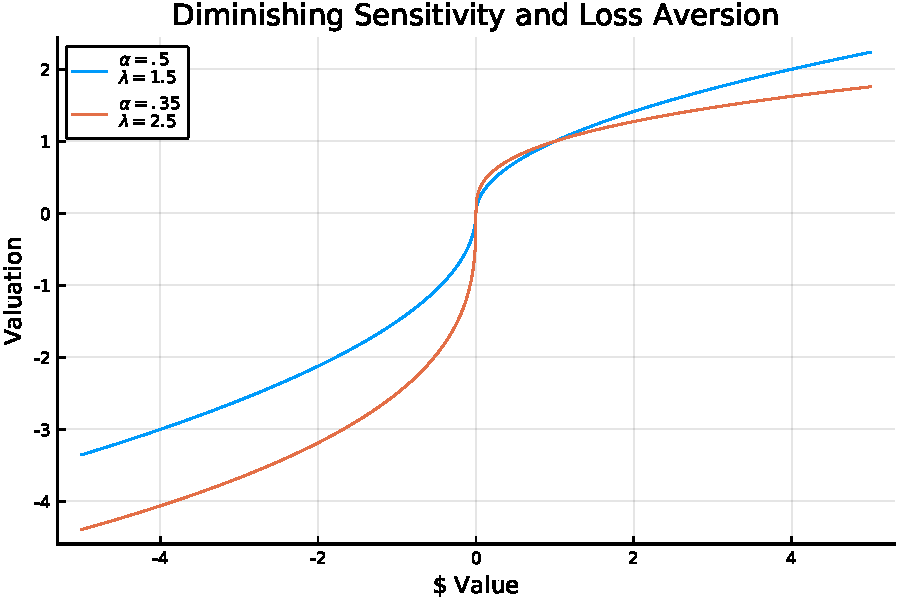
\includegraphics[width=.75\linewidth]{../Plots/ValueFunction.pdf}
\end{center}

In cumulative prospect theory, the cumulative mass (distribution)
function is weighted such that individuals overweight the tail
probabilities. This is especially important in this model, as there are
many high valued rare items. If this is the case, a severely distorted
distribution could lead to individuals systematically overvaluing
lotteries despite even being risk-averse. Colloquially, it is believed
that this concept is what allows for this type of randomization to
flourish in a market that is primarily populated by young people.

\begin{equation*}
  w(P) = \frac{ \gamma P^\delta }{ \gamma P^\delta + (1-P)^\delta }
\end{equation*}

Following the intuition provided by \cite{GONZALEZ1999129}, $\delta$
captures the notion of diminishing sensitivity,
and $\gamma$ captures attractiveness. Diminishing sensitivity captures how
individuals discriminate cumulative probabilities away from the
endpoints, i.e. the curvature of the weighting
function. Attractiveness indexes how over or under-weighted certain
levels of cumulative probability are treated. It can be viewed as how
attractive a $50-50$ bet would be to a risk-neutral individual. It
captures the elevation of the probability weighting function.

A graph of different values of $\gamma,\delta$ and their affects on the
different weighting is shown. 

\begin{center}
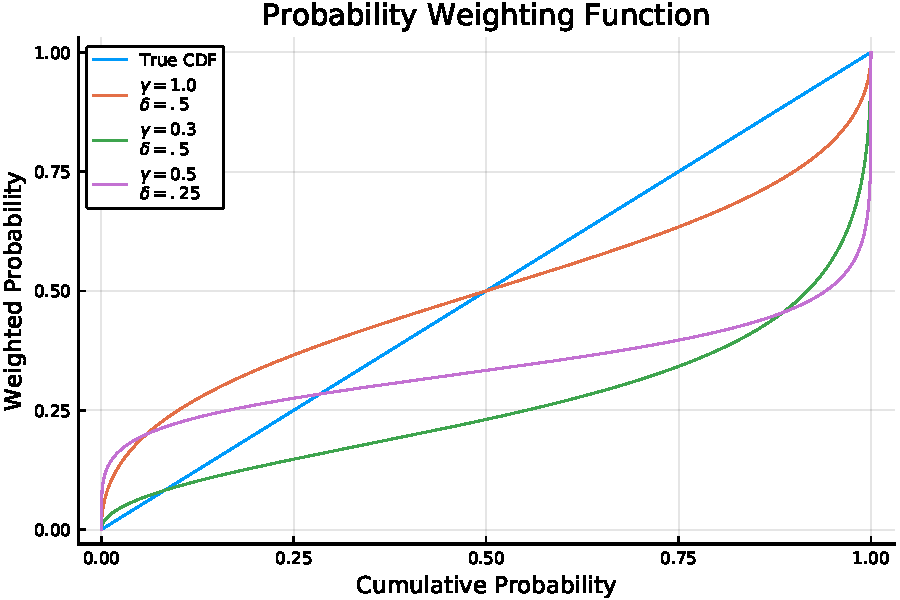
\includegraphics[width=.75\linewidth]{../Plots/WeightFun.pdf}
\end{center}




For some item that is within the contents of the box, a consumer's
valuation is transformed by the function:
\begin{equation*}
F(x_i) = \brak{w( \Pi_{s_i}) - w(\Pi_{s_i - 1}) } v( x_i - p_j - 2.50)
\end{equation*}

The valuation for the lottery can then be written as the sum of this
transformation for all of the contents of the lottery:

\begin{equation*}
  V(x,\pi,p_j) = \sum_{i=1}^K F( x_i)
\end{equation*}

\subsection{Constant Coefficient of Relative Risk Aversion}

Contrasting the behavioral aspects of this procedure is the use of a
Von-Neumann Morgenstern Utility function. However wealth level is not
observed, so following with the trends in the IO literature, we use a
Constant Coefficient of relative risk-aversion utility function to
capture an element of risk-aversion or risk-loving in the
individual.

Continuing with the quasilinear utility observed above, the individual
has utility of his current wealth if he elects not to buy the lottery,
and if he chooses to buy lottery $j$, his utility is given by:
\begin{equation*}
  U_{ij} = W_i - \beta p_j + \sum_{k=1}^{N_j} p_k \frac{x_k^{1-\alpha}}{1-\alpha}
\end{equation*}

The use of the CRRA utility function allows the wealth of the
individual to not be present in his valuation of the lottery, so that
wealth only appears linearly in the utility function. As a result,
when looking at the maximum between many lotteries, we can remove
wealth from the equation. I posit that the utility of an individual
that chooses lottery $j$ at time $t$ can be given by:

\begin{equation*}
  \sum_{k=1}^{N_j} p_k \frac{x_k^{1-\alpha}}{1-\alpha} - \beta p_{jt} + \xi_{jt} + \epsilon_{jt} 
\end{equation*}

Where $\epsilon_{jt}$ is a type-1 extreme value distribution, and $\xi_{jt}$
are the unobserved characteristics of the lottery. Thus this model
follows Berry (1994), but infers a different valuation function for the
lottery using a CRRA utility function and subtracting some level of
wealth. This allows for the same estimation strategy to be used for
the rational case as the behavioral model. 



\section{Estimation}

\subsection{Estimation}

In all formulations of the model, it can be written as:

\begin{align*}
  \xi_{jt} = \log s_{jt} - \log s_{0t} - \beta' C_j - V( x_{jt}, p_{jt}; \theta)
\end{align*}

Where $C_j$ are the observed characteristics of the lottery, $\xi_{jt}$
are the unobserved characteristics of the model, $s$ are the market
shares at a given time, and $\theta$ are the model parameters.

Estimation of this model proceeds using the least-squares
orthogonality conditions of $\exV{\xi_j Z_j} = 0$. Since I have made
no distributional assumptions on $\xi_{jt}$ I shall conduct this
estimation using the generalized method of moments. The matrix of
$Z_j$ is constructed from the exogenous prices of the contents of the
lotteries, but also from the price instruments, and the exogenous
active buy order price terms. 

Consider a matrix of exogenous variables $Z_j$ defined as above, we wish
to estimate the parameters of $V$ based on the condition that this
matrix is orthogonal to $\xi$. This could be accomplished using either
Nonlinear Least-Squares or Generalized Method of Moments, I shall
employ the latter.

All of the orthogonality conditions combine to:
\begin{equation*}
  \exV{Z_{jt}'\xi_{jt}} = 0
\end{equation*}

The estimation procedure can be written as:

\begin{align}
  &\min_{\bm{\xi}_{j,t}, \xi_{j,t}, \beta_0, \theta} \sum_{j,t}\bm{\xi}_{j,t}' \Omega \bm{\xi}_{j,t}\\
  \text{subject to: } &\xi_{j,t} = \log s_{jt} - \log s_{0t} - \beta'C_j
                        - V( x_{jt}, p_{jt}; \theta)\\
  &\bm{\xi}_{j,t} = \xi_{j,t} \bm{Z}_{j,t}  
\end{align}

Note that $C_j$ contains a constant term that incorporates the
expected value of $\xi$ and the normalization utility of the outside
option. We will not interpret it as meaningful Economically. For the
weighting matrix $\Omega$, we follow the standard of using the two-stage
least-squares weighting matrix $\inv{Z'Z}$. From this estimate, I
construct the two-stage estimator of the ideal weighting matrix. The
model is estimated again using the two-stage weighting matrix, and
point estimates as well as estimates of the standard errors. 

I examine four different variations of the behavioral model. I
consider two different reference points, one of which is taken as
simply the price that a consumer pays, where gains are taken as
any return that is strictly above threshold, and losses below. The
other reference point is taken to be the price plus the expected value
of the loot box. This captures the notion that gains are not merely
gaining money, but relative to the expectations of the individuals
opening them. This notion cannot be made more precise with market
data, but there is room for expanding it with more precise
market-level data.

The other variants of the model arise from the characteristic vector
$C_j$, we examine the model when it only contains a single intercept,
and when it contains a separate intercept for each of the different
lotteries. This difference in the characteristics captures the
different characteristics of the lotteries that may account for the
heavy clustering present in the data. Since individual heterogeneity
is not present in this model, a large characteristic space is not as
computationally demanding as in the heterogeneous case.

Estimation is done using the programming language Julia, using the
software Julia for Mathematical Optimization. The Solver KNITRO is
employed, and the model estimation for $\approx 1200$ data points took
between four and eight hours for each specification. 


\subsection{Results}
The results for the four different variants of the cumulative prospect
theory model and the CRRA model are displayed below. The measure of
$\bar{R}^2$ used is $1 - \frac{\mathbb{V}(\xi)}{\mathbb{V}(Y)}$. This
captures the percent of the variation of the model that we are able to
explain. Standard errors are displayed in parenthesis.

We compute both in-sample and out-of-sample RMSE to capture any
notions of over-fitting, and report the J-statistic as well. The
critical values for the J-statistic are as follows:
Fixed Effects: 5\% 314.6784, 1\% 332.4796
No Fixed Effects: 5\% 337.1254, 1\% 355.5251

\begin{minipage}{\linewidth}
  \centering
    \captionof{table}{Point Estimates}
  \scalebox{1.0}{%
\begin{tabular}{@{}cccccc@{}}\toprule
  \multicolumn{3}{c}{$\exV{V}$ + Price Reference Point} & &\\
\cmidrule{1-3}
$\alpha$ & 0.56534 (2.03484) & $\lambda$ & 1.36844 (10.8477)\\
$\gamma$ & 1.0 (6.36280) & $\delta$ & 1.0 (9.47887)\\
  In Sample RMSE & 1.23649 & Out Sample RMSE & 1.4337\\
  $\bar{R}^2$ & 0.18880 & J-Statistic & 825.185\\
  \midrule
 \multicolumn{3}{c}{$\exV{V}$ + Price Reference Point and Fixed
  Effects} & &\\
\cmidrule{1-3}
$\alpha$ & 0.79549 (4.6084) & $\lambda$ & 0.60091 (9.85376)\\
$\gamma$ & 1.0 (9.79014) & $\delta$ & 1.0 (21.5814)\\
  In Sample RMSE & 1.08121 & Out Sample RMSE & 1.10642\\
  $\bar{R}^2$ & 0.51688 & J-Statistic & 558.41\\
  \midrule
\multicolumn{3}{c}{Price Reference Point} & &\\
\cmidrule{1-3}
$\alpha$ & 0.47457 (5.4068) & $\lambda$ & 0.54667 (14.56967)\\
$\gamma$ & 1.0 (10.97014) & $\delta$ & 1.0 (10.85583)\\
  In Sample RMSE & 1.52584 & Out Sample RMSE & 1.5258\\
  $\bar{R}^2$ & 0.08117 & J-Statistic & 860.261\\
  \midrule
\multicolumn{3}{c}{Price Reference Point and Fixed Effects} & &\\
\cmidrule{1-3}
$\alpha$ & 0.8215 (7.6682) & $\lambda$ & 0.3152 (7.3252)\\
$\gamma$ & 1.0 (7.6753) & $\delta$ & 1.0 (15.7306)\\
  In Sample RMSE & 1.01432 & Out Sample RMSE & 1.07900\\
  $\bar{R}^2$ & 0.54053 & J-Statistic & 351.73\\
  \midrule
\multicolumn{3}{c}{Rational - CRRA} & &\\
\cmidrule{1-3}
$\alpha$ & 0.82589 ( 6093.657) & $\beta$ & -0.32488 (0.28937)\\
  In Sample RMSE & 0.98513 & Out Sample RMSE & 1.10097\\
  $\bar{R}^2$ & 0.52163 & J-Statistic & 570.394\\\bottomrule
\end{tabular}
}
\end{minipage}

\vspace{.2in}

We reject the Null that the model is correctly specified in all cases,
though the fixed effect does come close. Although this is not
troubling as the mode is incredibly over-identified, it suggests that
there is variation in the prices that the consumers are not sensitive
to under these specifications. This suggests that a more
non-parametric approach may be able to better explain variations in
the data. At the very least, there is some misspecification in the
models employed.

We can see that there is relatively little of the variation in the
quantities explained by simply the valuations, and without fixed
effects we have a very small $\bar{R}^2$ level for the cumulative
prospect theory. This may indicate that the prices that individuals
are sensitive to may not be the last posted price, but some other
notion of price, possibly smoothed over time. Further work on this
topic should focus on this aspect, as well as relaxing the
assumptions of homogeneity for a more complex model.

The standard errors of each of the estimates that appear in the
lottery functions are very high. This occurs because of the
extremely over-identified model and the dense Jacobian used to
calculate the standard errors. These errors do not reduce upon further
iterations of the weighting matrix. Since each term in the behavioral
model enters the valuation function in an extremely non-linear manner,
the Jacobian is poorly approximated by a quadratic function, and thus
standard errors constructed will be extremely high. 

The estimate of the model using a CRRA utility function produces a
curious result. I find a strong level of risk aversion. There
is such a large standard error tough that the possibility of risk
neutrality or risk-loving nature cannot be ruled out. This basic
utility function which is quite parsimonious allows for just as
strong of a fit both in sample as out-of-sample as the model based on
cumulative prospect theory.

None of the behavioral models suggest that probability weighting is
being exhibited. In all formulations of the model, individuals simply
slightly differently weigh losses and the convexity of gains. This
suggests that the result that individuals do not use probability
weighting is quite robust to model miss-specification. I note that I
do place constraints on $\gamma,\delta$ such that they are bounded between $0$
and $1$, and limit $\delta$ to a slightly higher value than $0$ purely for
numerical reasons. This ensures that we would not see under-weighting
of the probability weighting functions, and thus I only allow for
over-weighting.

The concavity of the valuation function combining with the lack of
probability weighting shows that risk-aversion is what is suggested by
the cumulative prospect theory models as well. In fact, these
specifications all report a negative valuation under cumulative
prospect theory. In this framework, individuals are aware that
they face a losing bet, but they obtain some fixed level of utility
for participating in the lottery. This ``fixed effect'' drives
purchases, and can only be interpreted as utility from the act of
gambling, completely independent of the potential rewards.

While market equilibrium between the different cases was employed in
the estimation of the model, the equilibrium between the prices of the
contents of the cases and the prices of the cases was never used. This
creates an interesting outside-moment condition where I can examine
how each model fits this equilibrium condition. I consider the
equilibrium condition as indifference between the valuation of the
lottery and the price of the lottery. This is all encompassed in the
valuation function for the cumulative prospect theory models, but are
two separate terms in the rational model. In both I take the average
over each data point and consider which is closer to zero. I consider
both the case of market transactions only, and market transactions and
buy orders for the behavioral model, and report the average over all
data points for the rational. 

\begin{minipage}{\linewidth}
  \centering
  \captionof{table}{Lottery Valuations}
  \begin{tabular}{@{}lcccccc@{}}\toprule
    & \multicolumn{2}{c}{Characteristics} & &\multicolumn{3}{c}{Lottery Valuations}\\
    \cmidrule{2-3} \cmidrule{5-7}
  Case & $\mathbb{E}[V]$ & Price &\quad& CPT Valuation & Market Only & Rational\\\midrule
Operation Breakout & 0.77011 & 2.5305 &\quad& -0.40693 & -0.40693 & -0.0052805\\
Operation Wildfire & 0.89891 & 2.5307 &\quad& -0.32827 & -0.32827 & -0.0049704\\
Huntsman Weapon Case & 0.95531 & 3.3181 &\quad& -0.49249 & -0.53162 & -0.15657\\
Shadow Case & 0.85299 & 2.5349 &\quad& -0.35231 & -0.3512 & -0.0059236\\
Falchion Case & 0.95072 & 2.5323 &\quad& -0.36465 & -0.36465 & -0.0063908\\
Chroma Case & 0.83215 & 2.55 &\quad& -0.34827 & -0.34559 & -0.0095399\\
Chroma 2 Case & 1.0058 & 2.53 &\quad& -0.33199 & -0.33199 & -0.0048381\\
Spectrum Case & 0.98146 & 2.53 &\quad& -0.24042 & -0.24042 & -0.005158\\
Chroma 3 Case & 0.66099 & 2.53 &\quad& -0.38344 & -0.38344 & -0.0053253\\
Operation Hydra & 1.5465 & 4.0827 &\quad& -0.18677 & -0.31092 & -0.24581\\
Glove Case & 0.84301 & 2.53 &\quad& -0.31471 & -0.31471 & -0.0051815\\
Gamma 2 Case & 0.68335 & 2.53 &\quad& -0.34373 & -0.34373 & -0.0053237\\
Gamma Case & 0.80717 & 2.53 &\quad& -0.28795 & -0.28795 & -0.0052006\\
CS:GO Weapon & 4.4611 & 9.3248 &\quad& -0.20035 & -0.63434 & -1.5106\\
eSports 2013 Case & 3.2708 & 10.354 &\quad& -0.34529 & -1.0796 & -1.2112\\
eSports 2013 Winter & 1.5687 & 2.6441 &\quad& -0.081838 & -0.058941 & -0.037442\\
Operation Phoenix & 0.85507 & 2.5416 &\quad& -0.35965 & -0.35737 & -0.0089612\\
Winter Offensive & 1.299 & 3.5079 &\quad& -0.38325 & -0.43248 & -0.19626\\
Operation Vanguard & 1.038 & 2.5928 &\quad& -0.35491 & -0.34876 & -0.021628\\
Operation Bravo & 4.3567 & 12.628 &\quad& -0.74652 & -1.2878 & -2.3076\\
eSports 2014 Summer & 1.4136 & 2.7414 &\quad& -0.22718 & -0.21321 & -0.059558\\
Revolver Case & 1.1045 & 2.53 &\quad& -0.27059 & -0.27059 & -0.0046285\\\bottomrule
  \end{tabular}
  
\end{minipage}
\vspace{.2in}



The rational model presents a much more compelling story. Although it
provides risk-aversion, the high sensitivity to price allows for the
valuations of the lotteries to be closer to zero than the cumulative
prospect theory estimates. The average over all lotteries is $-0.2647$
compared to $-0.33416$ for the cumulative prospect theory. However the
rational model appears to have several outliers that influence the
mean heavily. If we consider the more robust median we get a median
valuation estimate of $-0.007676$ for the rational case and $-0.34451$
for the behavioral model. Appealing to market equilibrium, we find that
the rational model is actually predicting behavior better than the
behavioral model. The outliers themselves occur for the lotteries for
which there is a high price relative to the other lotteries, and the
poor fit is likely explained by poor price instruments, which are more
relevant in the CRRA model where price appears linearly. 

Alternatives to explore this range from the models of Belief
Heterogeneity utilized by Bajari, to adding preference heterogeneity
and non-parametric fit, as used by others. Another alternative is
changing how the price of the contents is computed, using averages
over the past rather than simply the spot price on the day the lottery
was sold. However many of these options are much more computationally
intensive, and may require simplifications in other aspects of the
model to be able to be computed.

\section{Conclusion}

Although there is high uncertainty in our estimates in any
specification of the model, it is not clear that there is substantial
information to be gained from application of the behavioral model of
cumulative prospect theory to market level data. It appears that
market shares are less determined by the valuations of the lotteries
under any specification than other characteristics. That is, in this
market individuals are less price sensitive than they are sensitive to
the other characteristics present in the market. In fact, when
examining which model better represents equilibrium between the
contents and the lottery itself, the rational model predicts better
than the behavioral model.

This suggests individuals are less price sensitive to their valuations
when opening lotteries than they are to the price of being able to
open the lottery, based on the computed price sensitivity from the
rational case. It is difficult to determine price sensitivity for
cumulative prospect theory, as the price is embedded in the model in a
more complex notion, so determining a distribution is computationally
taxing. 

If a behavioral model is to be adopted, the reference point used
appears to be quite sensitive to model misspecification. This makes
utilization of this model in market situations less appealing, as
unobserved characteristics will always be present in structural
estimation from market data. This paper is unable to build intuition
or guidance for the choice of an ideal reference point, as it is
unclear from the results which reference point from the two examined
is more informative.

Cumulative Prospect Theory has aided many researchers in the
laboratory, but its use in the field has been limited due to many
complexities in the data. This foray into market data suggests that
its ability to explain deviations is limited compared to simple models
of choice under uncertainty, and adds significant computational
complexity that precludes more complicated models of heterogeneity. I
find that it is not worthwhile when examining lotteries at the market
level to use cumulative prospect theory, due to the large increases in
computational power and lack of external validity in outside moment
conditions. 



% I intend to estimate a structural model for the demand for the
% contents of the boxes, using this, we can determine the distribution
% of valuations for a risk-neutral consumer for the boxes, and then
% estimate the risk-preference of the individuals that open the
% loot-boxes. From there we can calculate the benefit of randomization
% compared to selling each item at market.

%  \subsection{Demand Estimation}

% We wish to estimate the demand for this model using a discrete choice
% model for demand. This immediately raises the concern that it only
% allows for one good to be purchased, and it is common for individuals
% to have many weapon skins in the game. To this end, we shall split the
% market into several sub-markets and make a heavy identifying
% assumption. This assumption will allow for the discrete choice model
% to be applicable, and also creates price instruments for estimation.

% \begin{assume}
%   Items are split into markets defined by the in-game role that all of
%   the weapons in this market fulfill.
% \end{assume}

% These markets are defined by domain knowledge. For example, we treat
% the AK-47, the single most popular gun in the game as its own market,
% competing only with its own skin and condition variants. However, the
% M4A4 and the M4A1-S will be considered as competitors, as will the
% CZ75, Tec9, and Five-Seven. Weapons that fill the same role, or the
% same weapon slot will be considered in the same market. The assumption
% takes the form of claiming that one individuals do not substitute
% between roles, and only consider substitution between weapon skins for
% the same role. This ensures that consumers only purchase a single item
% at a time, as one could never equip multiple skins for the same
% role. The full power of this assumption will become clear in the
% instruments section.

% \subsubsection{BLP}

% To estimate the demand for the contents of the boxes, I intend to
% implement a standard BLP demand estimation model (1995). This is a discrete
% choice demand system. Consider $J$ goods in $T$ markets for $I$
% consumers indexed by $j,t,i$ respectively. Assuming quasilinear
% utility, the utility for consumer $i$ purchasing good $j$ is:

% \begin{equation*}
%   u_{ij} = \alpha_i p_j + x_j \beta_i + \xi_j + \epsilon_{ij}
% \end{equation*}

% Where $p_j$ is the price of good $j$, $x_j$ are the observed
% characteristics of good $j$, $\xi_j$ are the characteristics of good
% $j$ observed by consumers and producers but not by the econometrician,
% $\alpha_i, \beta_i$ are consumer i's individual preference parameters over
% these characteristics, and $\epsilon_{ij} \sim T1EV(0)$ is a random shock only
% observed by the consumer. This is a standard logit model, but we have
% unobserved heterogeneity among consumers.

% Consumer $i$ then chooses the good that gives him the highest utility,
% the probability that that good is good $j$ is given by:
% \begin{equation*}
%   \Pr( i \rightarrow j ) = \frac{\exp( \alpha_i p_j + x_j' \beta_i + \xi_j)}{\sum_{k \in
%       \mathcal{F}_t} \exp( \alpha_i p_k + x_k' \beta_i + \xi_k)}
% \end{equation*}

% Each consumer has individual logit demand. If we choose to normalize
% the mass of consumers to one, then the market share of good $j$ should
% be equal to the expected value of this individual demand, averaged
% over the distribution of valuations.

% \begin{equation*}
%   \pi_j = \exV{ \Pr( i \rightarrow j )}
% \end{equation*}

% Let us define the observed market shares as:
% \begin{equation*}
%   \hat{s}_j = \frac{1}{I} \sum_{i = 1}^I \indicate{y_i = j}
% \end{equation*}

% From the Weak Law of Large Numbers, we believe that $\hat{s}_j \plim
% \pi_j$. Define the distribution of $(\alpha_i, \beta_i)$ as $\theta$. By assuming that
% this convergence in probability has been reached, we arrive at:

% \begin{equation*}
%   \hat{s}_j \approx \exV{ \Pr( i \rightarrow j )} = \int \Pr( i \rightarrow j) d\theta \approx \frac{1}{N_s}
%   \sum_{i=1}^{N_s} \Pr( i \rightarrow j)
% \end{equation*}

% Where we approximate the integral of $\int \Pr( i \rightarrow j)d\theta$ through any
% numerical integration technique. This expression can then be inverted
% to solve for $\xi_j$, which is unobserved.

% \subsubsection{Instruments}

% In this specification of the model, there are two sets of endogenous
% variables. Price is obviously correlated with the unobserved
% characteristics of the model, but market share is also endogenous
% within the model. We shall require two sets of instruments, one for
% price, and one for market share.

% Valid price instruments are those that are correlated with supply
% shocks, but are not correlated with the demand shocks in the
% model. It is worth defining precisely what are the supply and demand
% for this model.

% The supply for each weapon skin is the set of people who have opened
% the loot box that contains that item and have elected to sell
% it. Shocks that will affect this are changes in consumer tastes
% leading to less people choosing to sell, as well as changes in the
% drop rates of the crates, controlling the flow of this item into the
% market.

% Demand for this good is the individuals who elect to buy the good at
% the market rather than attempt to earn it through opening loot
% boxes. The shocks that affect these people are entrance and exit to
% the market as well as changes in taste. (Needs more here)

% A Valid price instrument is something that is correlated with supply
% shocks, but not with the demand shocks. For this we will take the
% prices of the other contents of the box that are not in the same
% market as the good at hand. By Assumption 1, these prices are
% exogenous to the unobserved characteristics of the good at hand. They
% are however affected by the changes in the drop rate of the loot box
% that provides them, since they come from (nearly) the same
% supply. This is a form of the Hausman instruments used often in the
% literature.

% For market share, we intend to use the BLP instruments, which require
% that the valuation of one characteristic of a good is not random
% across the consumers. When this is satisfied, we may use the sum of
% the characteristics of the competitors of the good as instruments for
% the market share. If necessary, following \cite{OptimalBLPInstrument}, we
% may construct higher order approximations of the optimal instrument
% for the market shares using the observed characteristics.

% \subsubsection{Estimation}

% Once a set of instruments has been computed, estimation of the model
% requires using the orthogonality condition of the instruments against
% the computed values of $\xi_j$. Our orthogonality condition is:
% $\exV{\xi_j z_j} = 0$.

% This can be estimated using the generalized method of
% moments. Following the method of \cite*{MPEC}, we may estimate
% this using Mathematical Programming under Equality Constraints as
% follows: 

% \begin{align}
%   &\min_{\bm{\xi}_{j,t}, \xi_{j,t}} \bm{\xi}_{j,t}' \Omega \bm{\xi}_{j,t}\\
%     \text{subject to: } &s_{j,t} = \frac{1}{N_s} \sum_{i=1}^{N_s}
%                           \frac{\exp(\alpha_i p_j + x_j'\beta_i + \xi_j)}{\sum_{k\in
%                           \mathcal{F}_t} \exp( \alpha_i p_k + x_k'\beta_i +
%                           \xi_k)}\\
%   &\bm{\xi}_{j,t} = \xi_{j,t} \bm{z}_{j,t}  
% \end{align}

% This  method allows for the exploitation of sparseness in many
% commercial solvers. This is important as assumption 1 has imposed this
% level of sparseness on the model in part for computational ease.

% \subsection{Lottery Estimation Under Heterogeneity}

% Following the estimation procedure above nets estimates of the
% distribution of valuations that individuals in the market have for
% each of the items. However, the presence of the secondary market that
% they are able to re-enter complicates this, as any person with a
% valuation below the market price could simply sell their item on the
% market, earning that price. We shall take their valuations as the
% maximum between the observed market price and the estimate of the
% internal valuation. We shall refer to this maximum as $x_{ijt}$, or
% the valuation of consumer $i$ of content $j$ at time $t$

% However, if we were to estimate the lotteries and the demand
% separately, the model would be under-identified, as there would no
% longer be an exogenous variation in the lottery contents prices to
% provide identification of the different parameters of the lottery. The
% exogeneity we need must come from the demand estimation, and therefore
% the two procedures must be run simultaneously, ensuring a sense of
% equilibrium between the secondary market and the lottery market. 

% This essentially is adding another set of goods to the demand
% estimation, but requiring that the draws of their valuations come from
% the draws used in each of the ``roles'' in the demand estimation.  



% \section{Counterfactuals}

% Of interest is how much better this market structure is performing
% compared to a monopoly pricing schedule. This would require estimating
% the demand for the contents of the lottery, and then computing the
% optimal monopolist price for each good. 


% From these estimates, a monopoly pricing schedule that sets price
% where marginal revenue equals marginal cost for all goods can be
% computed, and its revenue compared to the revenue generated under the
% randomization scheme.


%\nocite{OptimalBLPInstrument}
%\nocite{SteamMarket}

\newpage

\section{Bibliography}

\bibliography{biblio}{}

\end{document}
